\documentclass[xcolor=dvipsnames]{beamer}
\usepackage[english]{babel}
\usepackage{hyperref}

\usepackage{amsmath}
\usepackage{amssymb}
\usepackage{xspace}
\usepackage{ltl} 
\usepackage{multirow}
\usepackage{calc}
\usepackage{tikz}
\usetikzlibrary{arrows,positioning,backgrounds,calc,shapes,decorations,automata,snakes}
\usetikzlibrary{mindmap}

\usefonttheme{professionalfonts}
\usepackage{appendixnumberbeamer}

\setbeamertemplate{sections/subsections in toc}[sections numbered]
\setbeamercolor{section in toc}{parent=normal text}
\setbeamertemplate{section in toc shaded}[default][60]
\setbeamertemplate{navigation symbols}{}

\usepackage{tcolorbox}

\usepackage{media9}
\usepackage{multimedia}

\makeatletter
%\setbeamertemplate{footline}[text line]{\strut\hfill\insertframenumber/\inserttotalframenumber\hspace*{1em}\hskip-\beamer@leftmargin}
\makeatother


\usepackage{stmaryrd}

\newcommand{\todo}[1]{\textcolor{red}{\textbf{TODO:}} #1\\}

\newcommand{\RM}[1]{{\textcolor{red}{ \textbf{RM:} #1 $\clubsuit$ }}}
\newcommand{\RD}[1]{{\textcolor{blue}{ \textbf{RD:} #1 $\spadesuit$ }}}
\newcommand{\LF}[1]{{\textcolor{magenta}{ \textbf{LF:} #1 $\spadesuit$ }}}
\newcommand{\HH}[1]{{\textcolor{brown}{ \textbf{HH:} #1 $\spadesuit$ }}}

\newcommand{\mcomment}[1]{}

\DeclareMathOperator*{\sign}{sign}

\newcommand{\ie}{i.\,e.\xspace}
\newcommand{\as}{a.\,s.\xspace}
\newcommand{\wlg}{w.\,l.\,o.\,g.\xspace}
\newcommand{\wrt}{w.\,r.\,t.\xspace}

\newcommand{\mc}[1]{\mathcal{#1}}
\newcommand{\reals}{\mathbb{R}}
\newcommand{\nats}{\mathbb{N}}
\newcommand{\set}[1]{\ensuremath{\{ {#1} \}}}

\newcommand{\pctl}{PCTL\xspace}
\newcommand{\pctlstar}{PCTL$^*$\xspace}
\newcommand{\ctlstar}{CTL$^*$\xspace}
\newcommand{\atlstar}{ATL$^*$\xspace}


\newcommand{\atoms}{AP}
\newcommand{\true}{\mathsf{tt}}
\newcommand{\false}{\mathsf{ff}}
\newcommand{\probX}{\mathbb{P}}
\newcommand{\pquant}{\probX^{\quantifierTiny}}
\newcommand{\pforall}{\probX^{\forall}}
\newcommand{\pexists}{\probX^{\exists}}

\newcommand{\bfx}{\mathbf{x}}
\newcommand{\bfe}{\mathbf{e}}

\newcommand{\init}{\iota}
\newcommand{\pprog}{(\bfx,C)}
\newcommand{\mdp}{(S,\rho)}
\newcommand{\dtmc}{(S^\alpha,\rho^\alpha)}
\newcommand{\Distr}{\mathit{Distr}}
\newcommand{\Supp}{\mathit{Supp}}
\newcommand{\Prob}{\mathit{Prob}}
\newcommand{\Paths}{\mathsf{Paths}}

\newcommand{\Pree}{\mathsf{Pre}_{\exists}}
\newcommand{\Pref}{\mathsf{Pre}_{\forall}}

\newcommand{\Player}{\mathsf{Player}}


\newcommand{\sem}[1]{[\![#1]\!]}
\newcommand{\Safe}{\mathsf{Safe}}
\newcommand{\Reach}{\mathsf{Reach}}
\newcommand{\Outcome}{\mathsf{Outcome}}

\newcommand{\at}{\mathit{at}}
\newcommand{\inm}{\mathit{in}}
\newcommand{\preserve}{\mathit{preserve}}

\newcommand{\close}{\mathit{close}}
\newcommand{\far}{\mathit{far}}
\newcommand{\origin}{\mathit{origin}}

\newcommand{\abs}[1]{|#1|}
\newcommand{\inv}[1]{#1^{-1}}

\newcommand{\sched}{\alpha}
\newcommand{\event}{\mathcal{E}}
\newcommand{\pevent}{\omega}
\newcommand{\indicator}[1]{[#1]}
\newcommand{\SampleSpace}{\Omega}
\newcommand{\SigmaAlgebra}{\mathcal{F}}
\newcommand{\Measure}{\mu}
\newcommand{\ProbabilitySpace}{(\SampleSpace, \SigmaAlgebra, \Measure)}
\newcommand{\CondProb}[2]{\mathbb{P}(#1 \; | \; #2)}
\newcommand{\Exp}[1]{\mathbb{E}(#1)}
\newcommand{\CExp}[3][{}]{\mathbb{E}^{#1}(#2 \; | \; #3)}
\newcommand{\Set}[1]{\{#1\}}
\newcommand{\SetCond}[2]{\{#1 \;:\; #2\}}

\newcommand{\qual}{\mathsf{qualitative}}
\newcommand{\quan}{\mathsf{quantitative}}
\newcommand{\infst}{\mathsf{Inf}}

\newcommand{\probOr}{\otimes}
\newcommand{\porder}{\succ}

\newcommand{\quantifier}{\protect\rotatebox[origin=c]{180}{\ensuremath{\mathrm Q}}}
\newcommand{\quantifierTiny}{\protect\rotatebox[origin=c]{180}{\tiny\ensuremath{\mathrm Q}}}
\newcommand{\nqRule}[1]{\ensuremath{\textsc{#1}}}
\newcommand{\qRule}[3][\quantifierTiny]{\ensuremath{\nqRule{#3}^{#1}}_{#2}}
\newcommand{\qDiscRule}[3][\quantifierTiny]{\ensuremath{\overline{\nqRule{#3}}^{#1}}_{#2}}

\newtheorem{appxprop}{Proposition}
\newtheorem{appxlemma}{Lemma}

% colors 
\definecolor{darkred}{rgb}{0.7 0 0}
\definecolor{lightred}{rgb}{1 0.2 0}
\definecolor{ired}{rgb}{0.8 0.36 0.36}
\definecolor{darkgreen}{rgb}{0 0.5 0}
\definecolor{darkblue}{rgb}{0 0 0.7}
\definecolor{lightblue}{rgb}{0.390 0.582 0.925}
\definecolor{darkgray}{rgb}{0.3 0.3 0.3}
\definecolor{gray}{rgb}{0.5 0.5 0.5}
\definecolor{lightgray}{rgb}{0.90 0.90 0.90}
\newcommand\bluet[1]{\textcolor{darkblue}{#1}}
\newcommand\magentat[1]{\textcolor{magenta}{#1}}
\newcommand\redt[1]{\textcolor{darkred}{#1}}
\newcommand\greent[1]{\textcolor{darkgreen}{#1}}
\newcommand\oranget[1]{\textcolor{orange}{#1}}


\newcommand{\colorize}[4]{\only<#1>{#4}\only<#2>{\textcolor{#3}{#4}}}

\newcommand{\colthree}[7]{
\only<#1>{\textcolor{#4}{#7}}
\only<#2>{\textcolor{#5}{#7}}
\only<#3>{\textcolor{#6}{#7}}
}
\newcommand{\coltwo}[5]{
\only<#1>{\textcolor{#3}{#5}}
\only<#2>{\textcolor{#4}{#5}}
}

\tikzset{
    invisible/.style={opacity=0},
    emph/.style={color=magenta},
    alert/.style={color=red},
    anotherhl/.style={color=blue},
    bold/.style={very thick},
    emph on/.style={alt={#1{emph}{}}},
    alert on/.style={alt={#1{alert}{}}},
    anotherhl on/.style={alt={#1{anotherhl}{}}},
    arrow on/.style={alt={#1{->}{}}},
    bold on/.style={alt={#1{bold}{}}},
    visible on/.style={alt={#1{}{invisible}}},
    alt/.code args={<#1>#2#3}{%
        \alt<#1>{\pgfkeysalso{#2}}{\pgfkeysalso{#3}} % \pgfkeysalso doesn't change the path
        },
    }
    
\newcommand{\ifstmt}{\underline{\text{if}}\ }
\newcommand{\thenstmt}{\ \underline{\text{then}}\ }
\newcommand{\elsestmt}{\underline{\text{else}}\ }
\newcommand{\assertstmt}{\textbf{assert}}
\newcommand{\uniform}{\textbf{Uniform}}
\newcommand{\bernoulli}{\textbf{Bernoulli}}
\newcommand{\boolt}{\underline{\text{bool}}\ }
\newcommand{\intt}{\underline{\text{int}}\ }
\newcommand{\doublet}{\underline{\text{double}}\ }

\newcommand{\modc}[1]{\text{mc}(#1)}

\newcommand{\SharpSAT}{\#SAT}
\newcommand{\SharpSMT}{\#SMT}

\newcommand{\SharpP}{\#P}
    

\begin{document}

\begin{frame}
\frametitle{Synthesis of surveillance strategies  {\small [submitted to ICRA'18]} \newline \small S.\ Bharadwaj, R. Dimitrova, and U. Topcu}

 Temporal evolution of uncertainty as a synthesis objective

\bigskip

\begin{center}
\begin{tikzpicture}[scale=1.6]
\draw[step=0.5cm,color=gray] (-2.5,-1) grid (1.5,1);
\filldraw[fill=red,draw=black] (0,0) rectangle (-0.5,-0.5);
\filldraw[fill=red,draw=black] (-0.5,0) rectangle (-1,-0.5);
\filldraw[fill=red,draw=black] (-0.5,0.5) rectangle (-1,0);
\filldraw[fill=red,draw=black] (0,0.5) rectangle (-0.5,0);

\uncover<1>{
\node at (1.25,0.75) {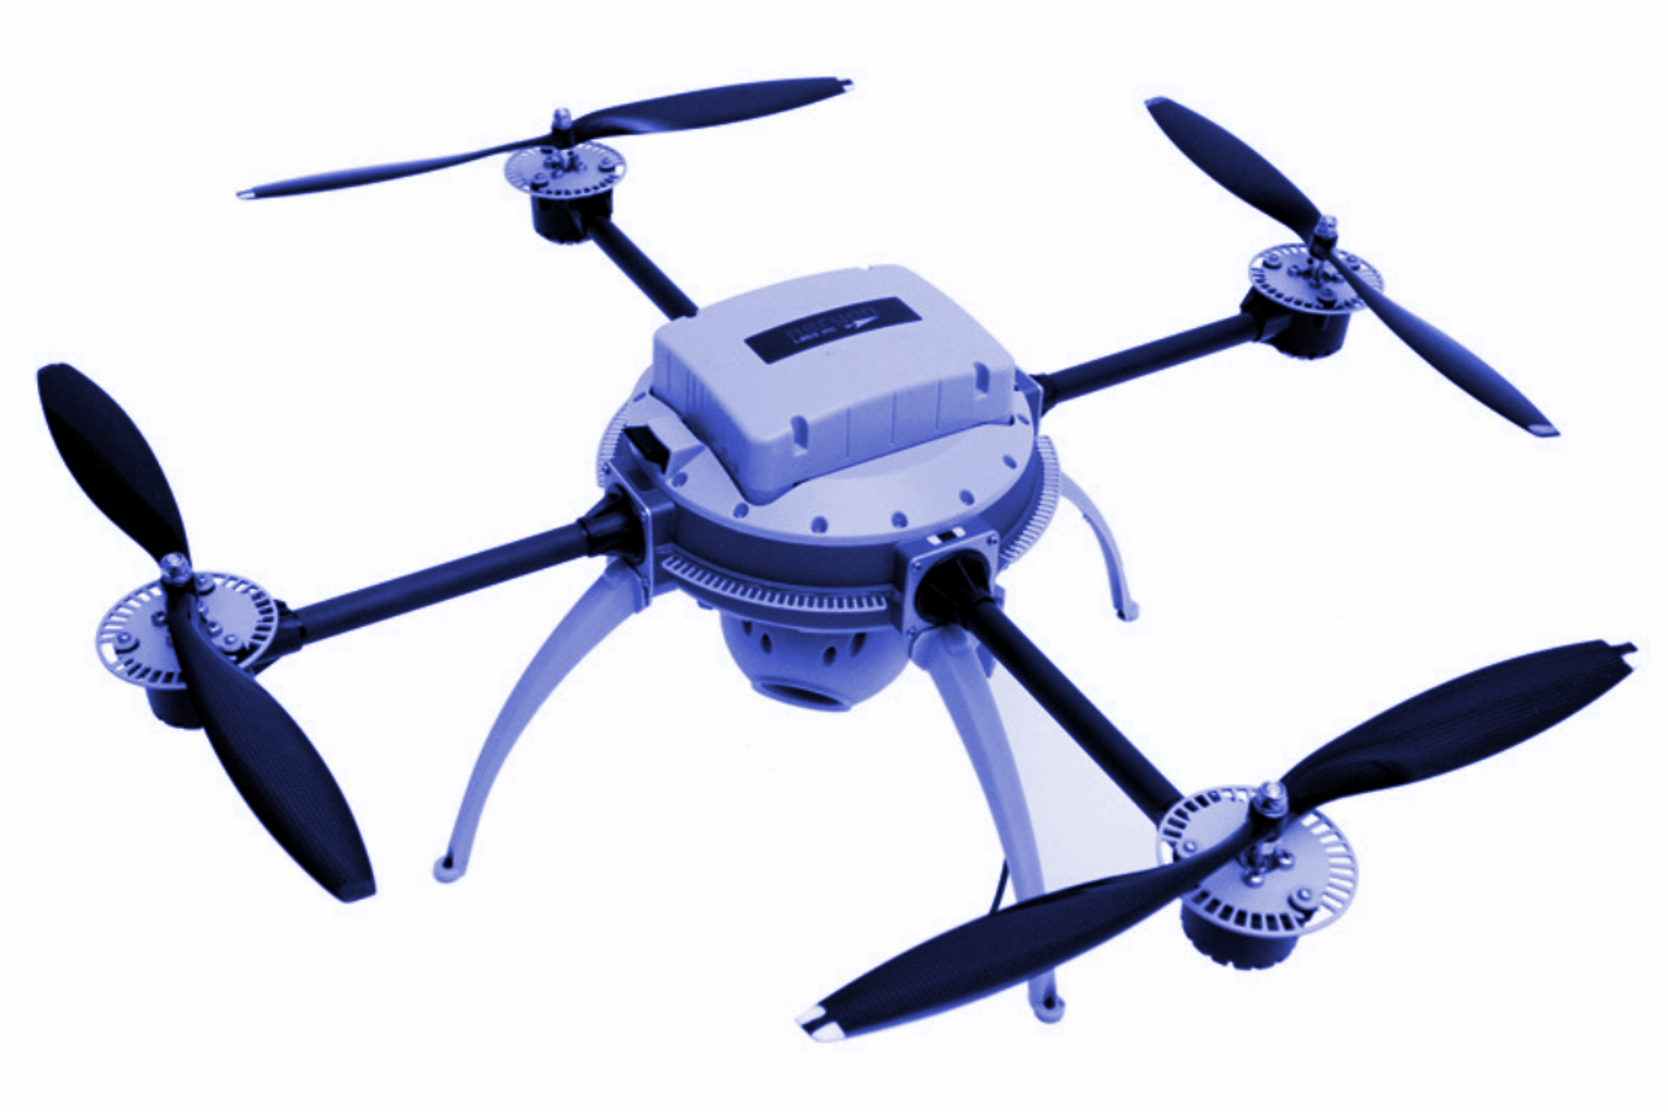
\includegraphics[scale=0.025]{./pics/agent.pdf}};
}
\uncover<2>{
\node at (0.75,0.75) {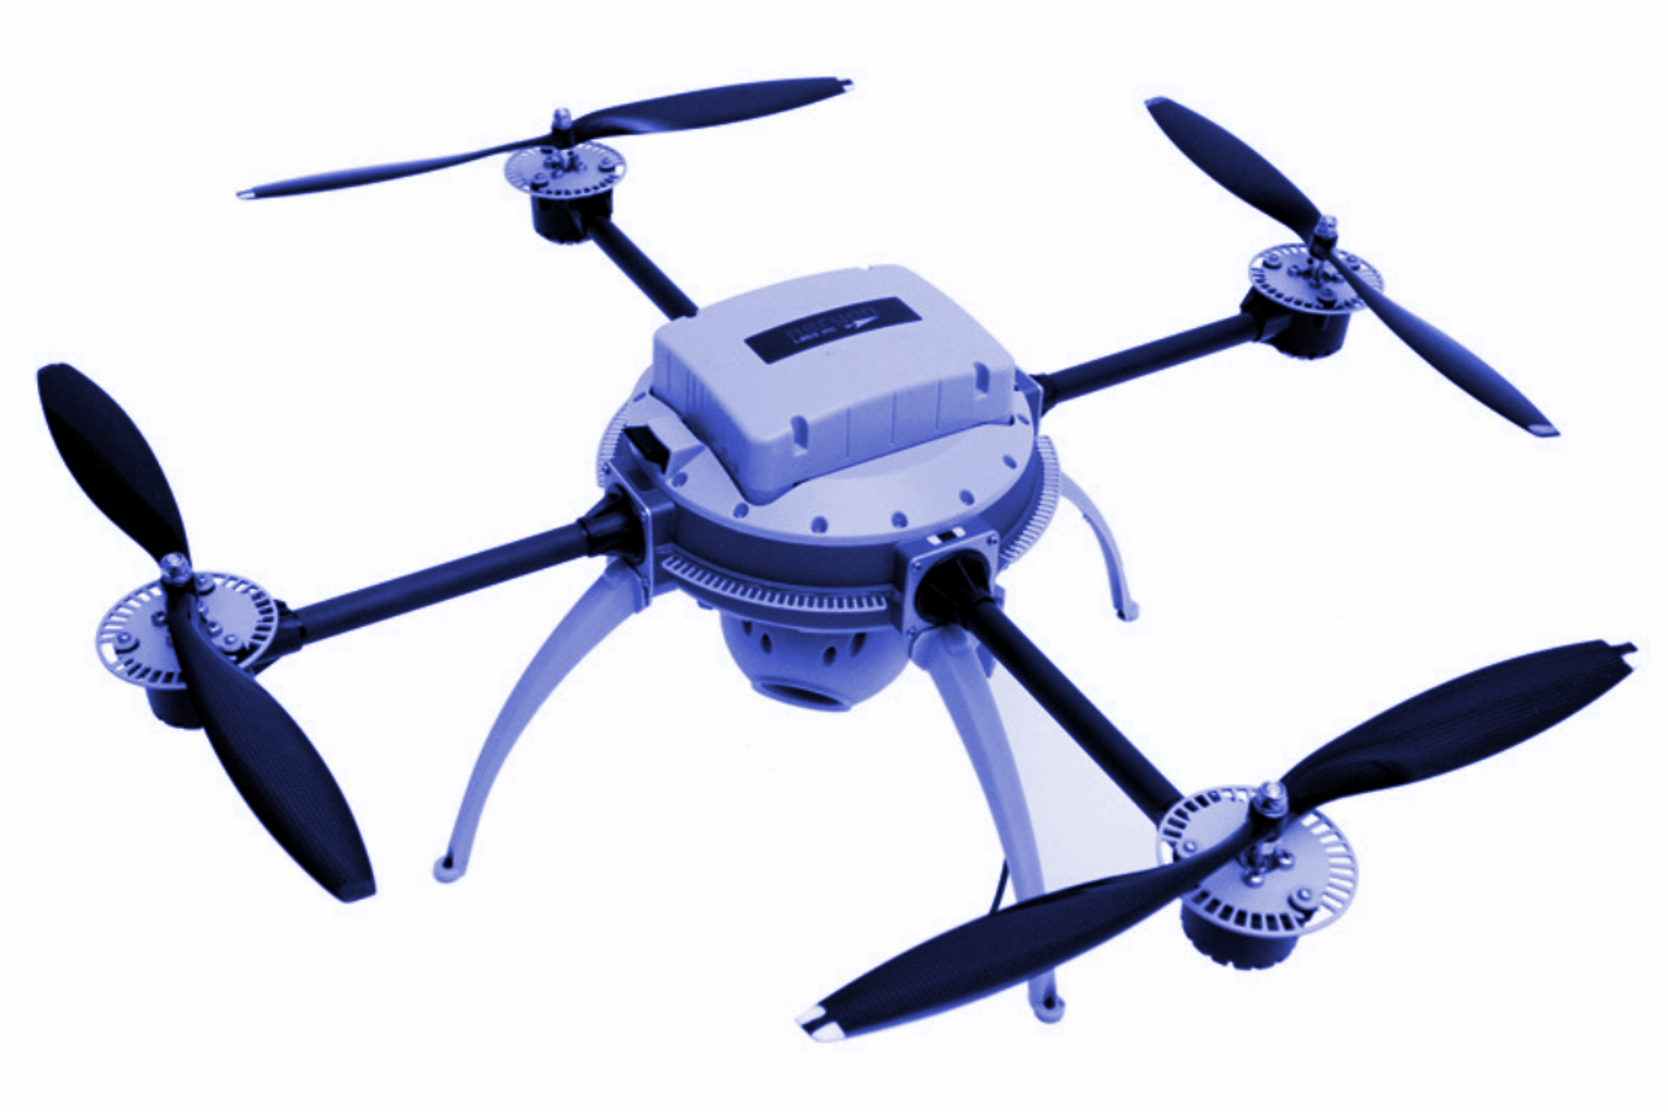
\includegraphics[scale=0.025]{./pics/agent.pdf}};
}
\uncover<3-4>{
\node at (0.25,0.75) {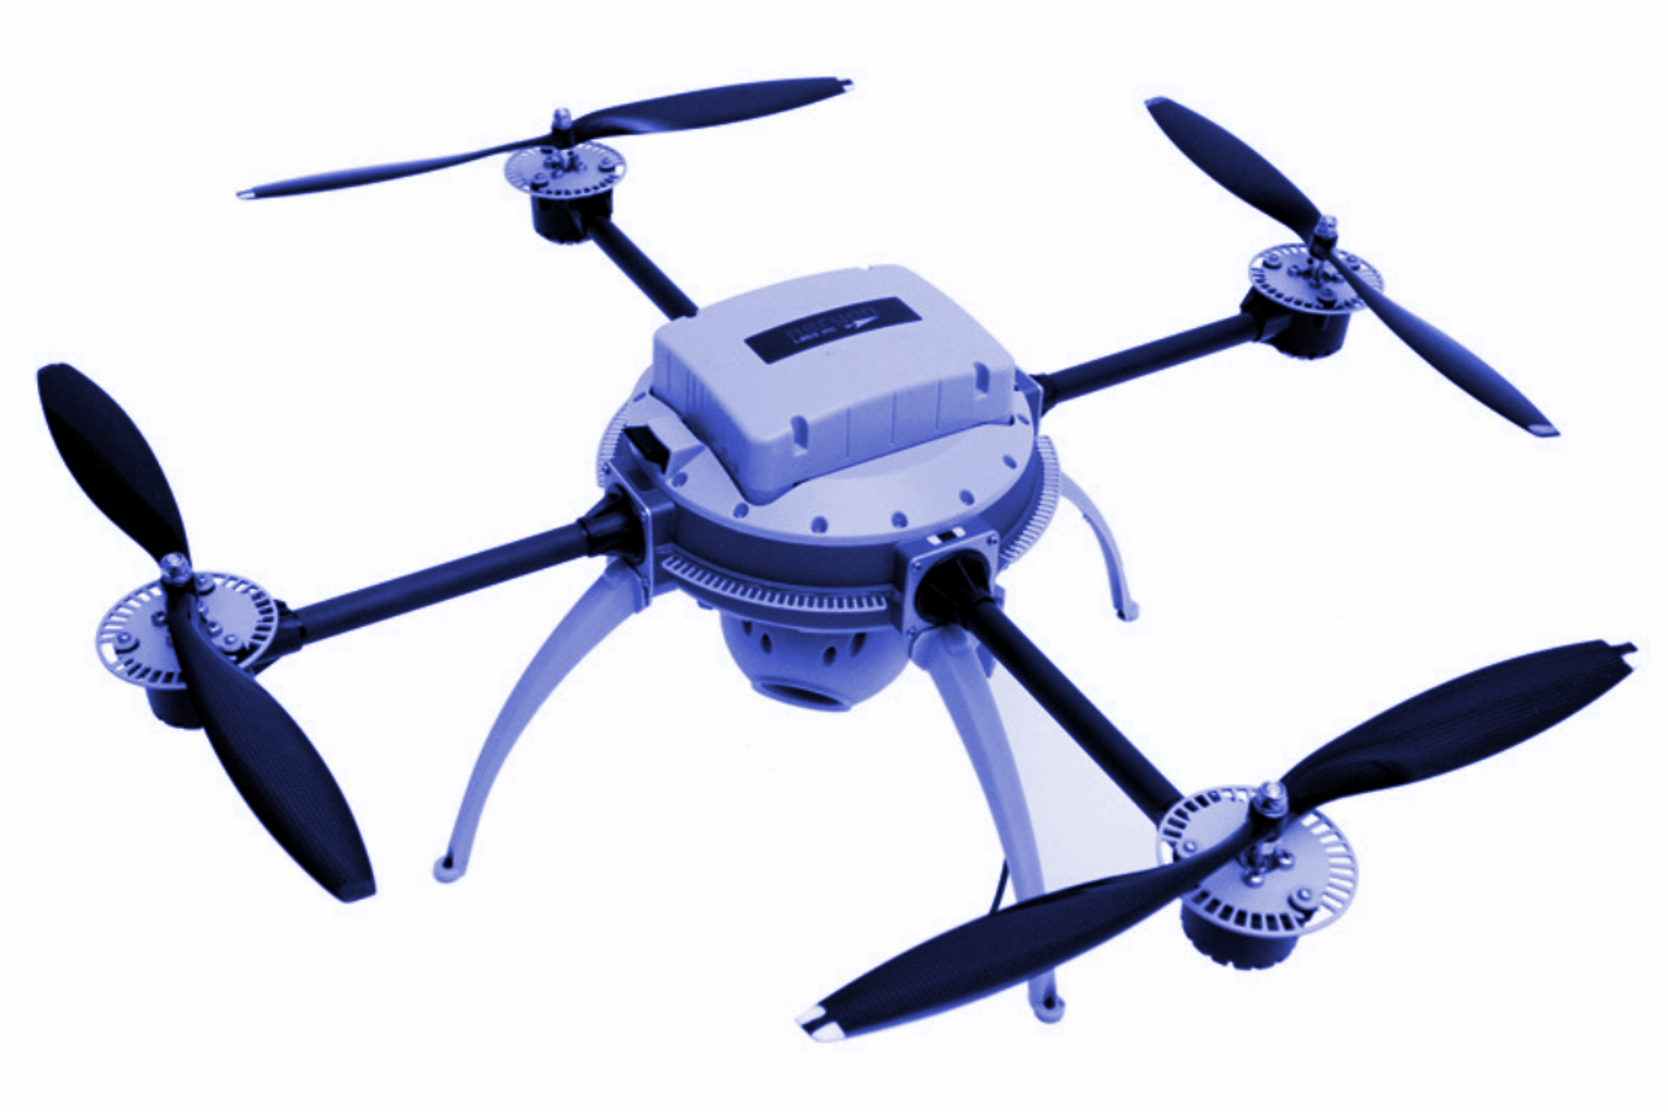
\includegraphics[scale=0.025]{./pics/agent.pdf}};
}
\uncover<1>{
\node at (-1.25,0.75) {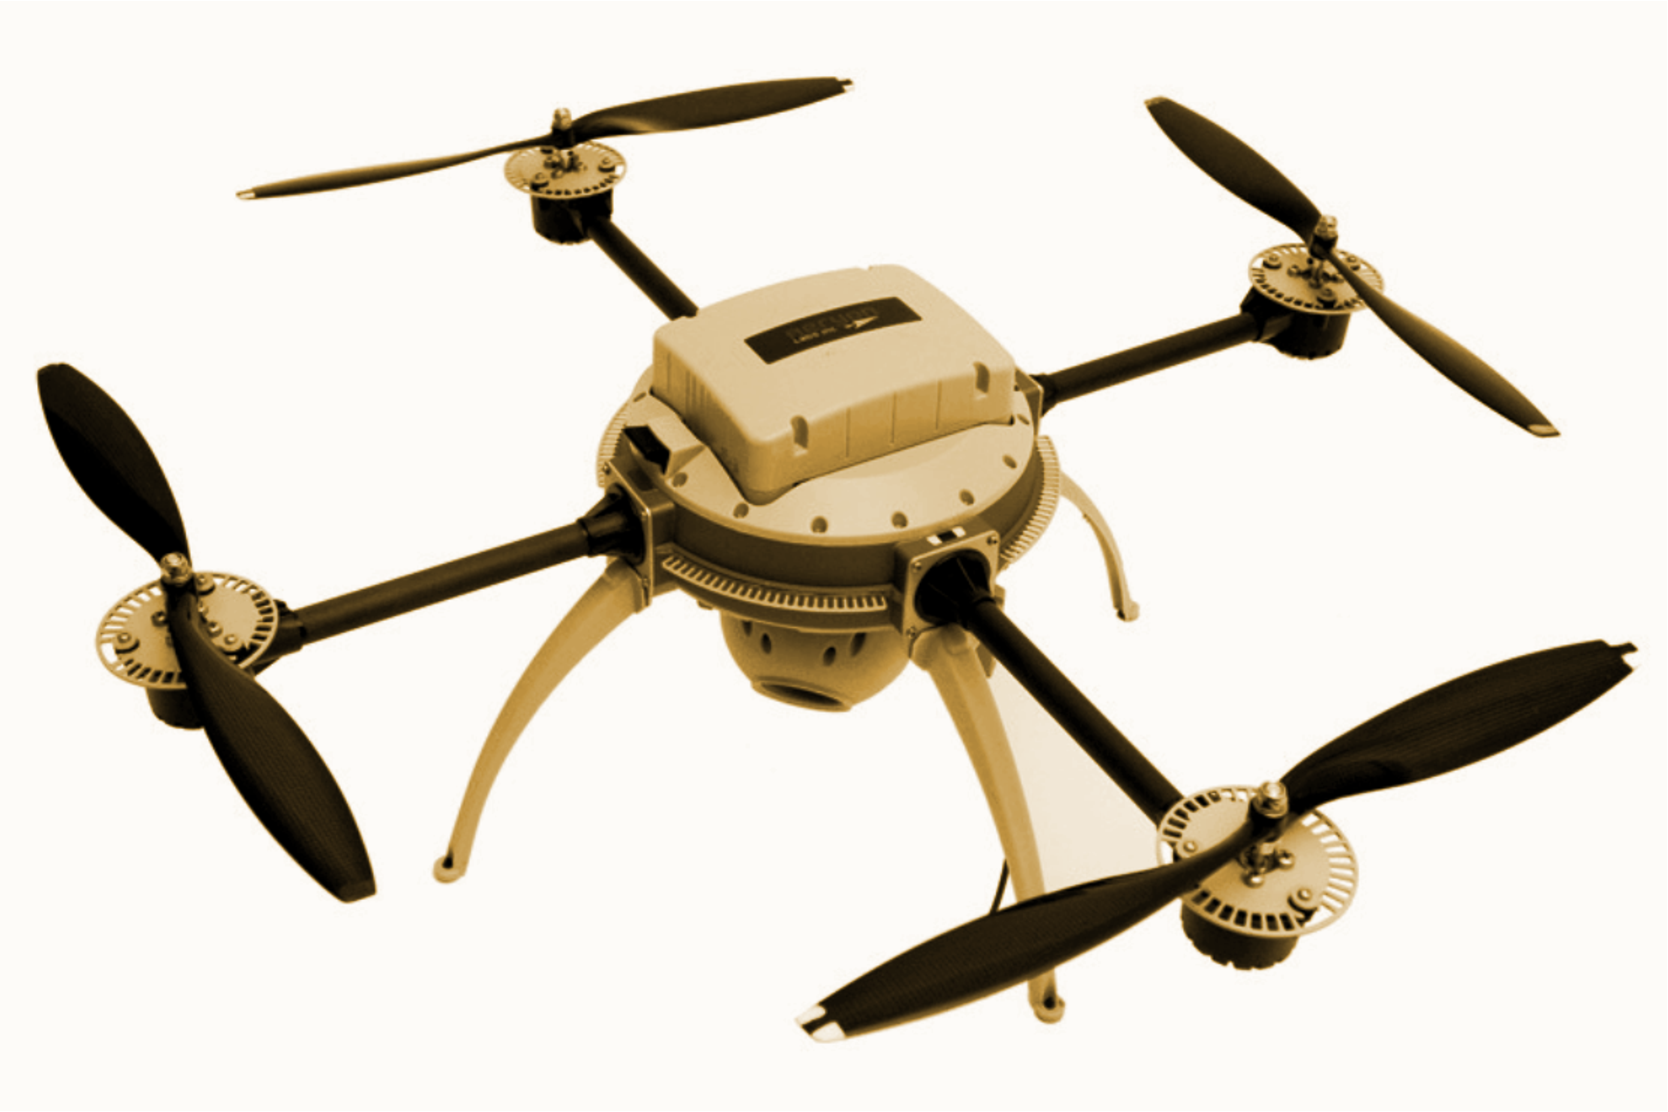
\includegraphics[scale=0.025]{./pics/target.pdf}};
}
\uncover<2>{
\filldraw[fill=white,draw=orange,very thick] (-1.5,0) rectangle (-1,0.5);
\node at (-1.25,0.25) {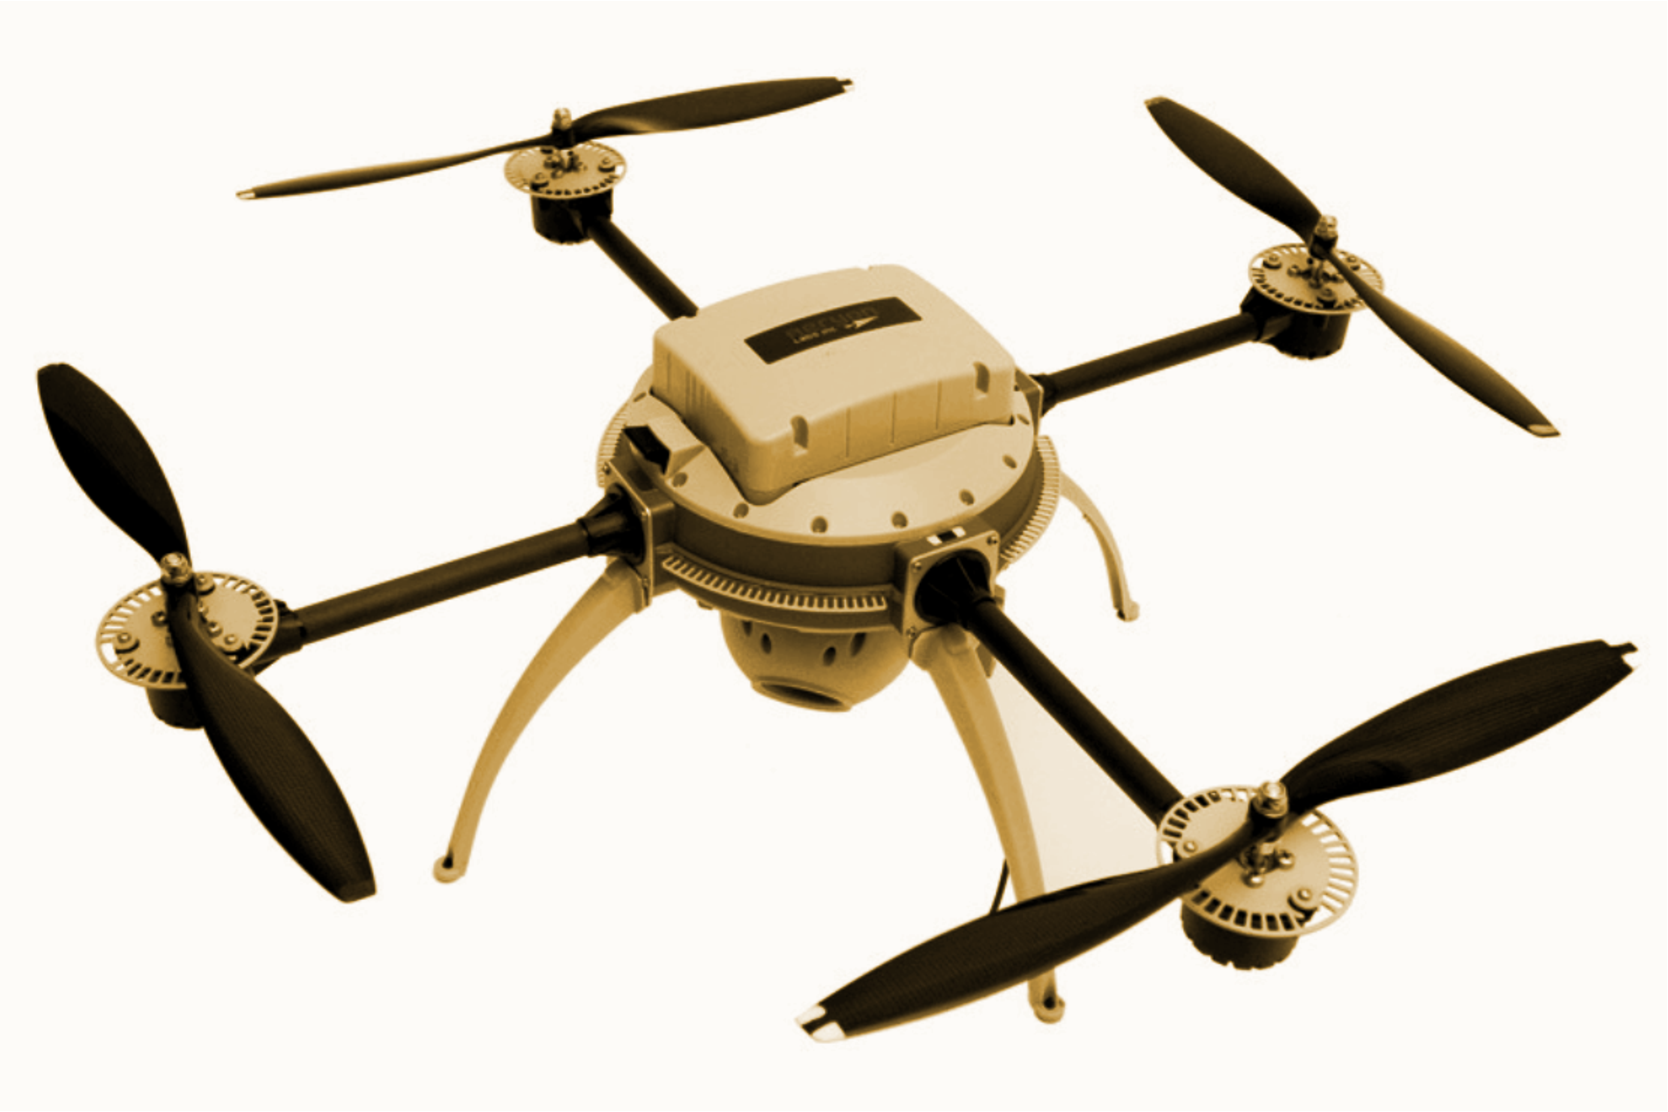
\includegraphics[scale=0.025]{./pics/target.pdf}};
}

\uncover<3-4>{
\filldraw[fill=white,draw=orange,very thick] (-1.5,0) rectangle (-1,0.5);
\filldraw[fill=white,draw=orange,very thick] (-2,0) rectangle (-1.5,0.5);
\filldraw[fill=white,draw=orange,very thick] (-1.5,-0.5) rectangle (-1,0);
\node at (-1.25,-0.25) {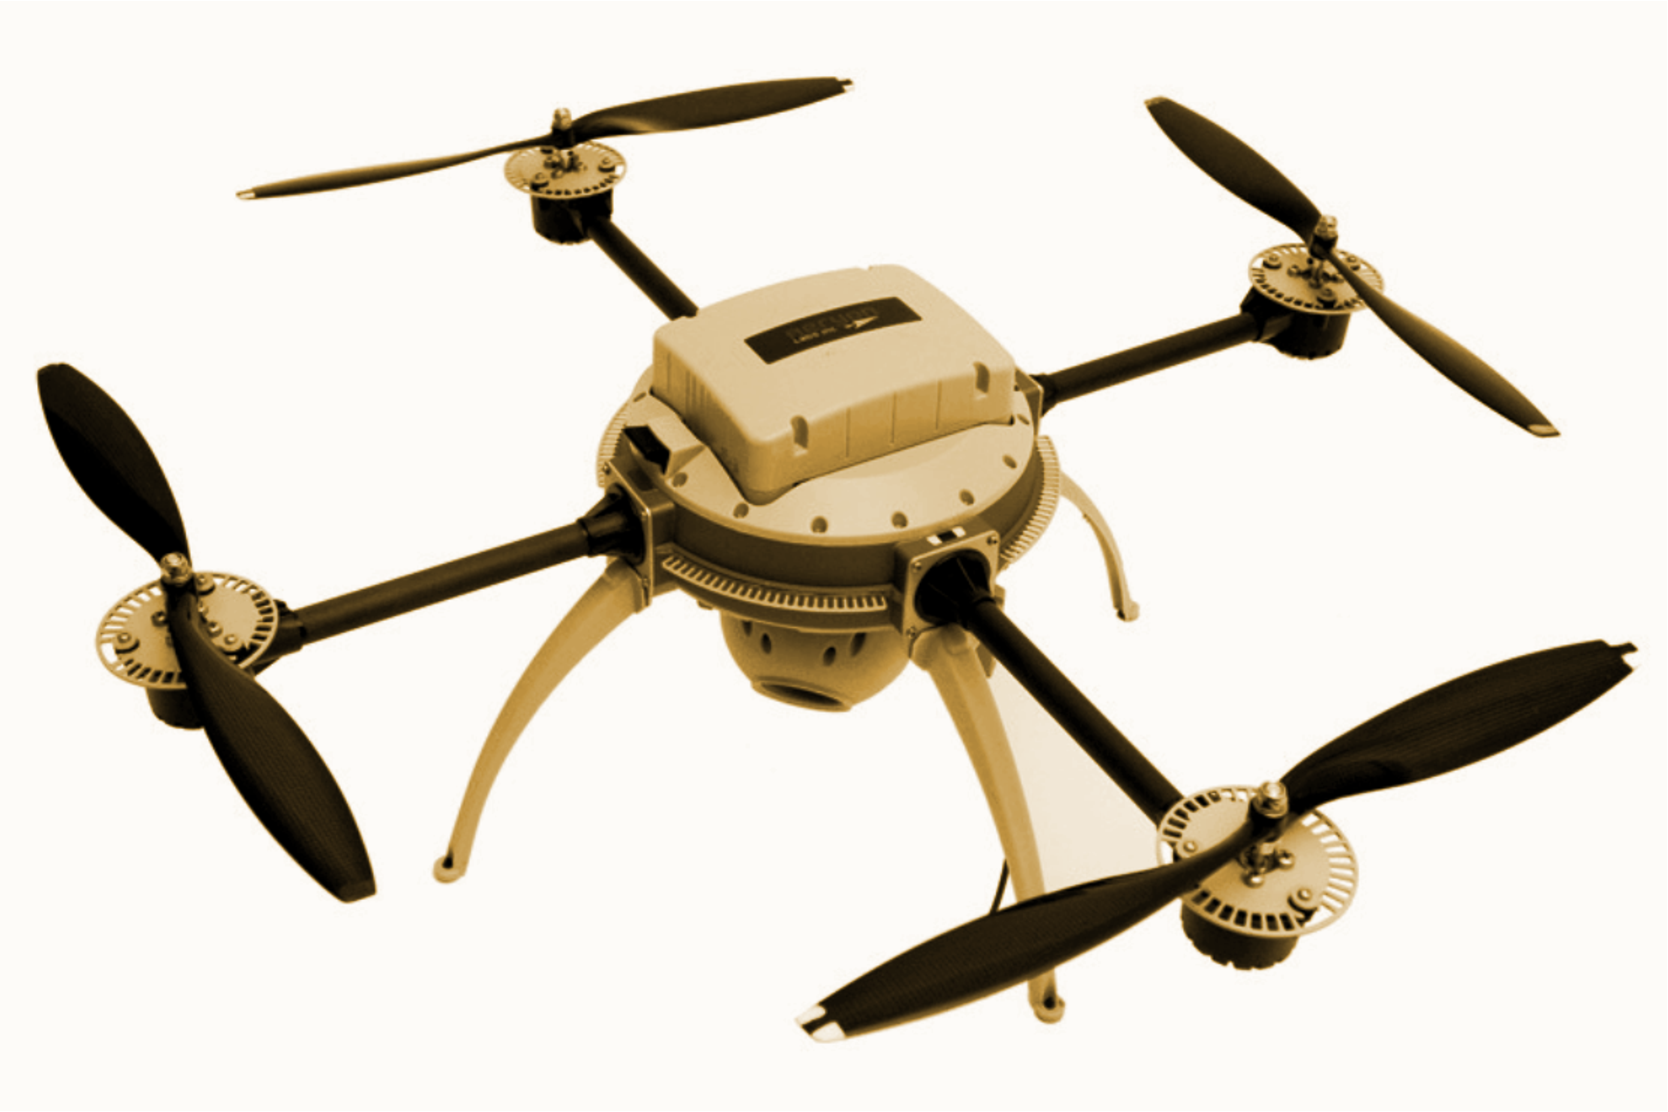
\includegraphics[scale=0.025]{./pics/target.pdf}};
}

\end{tikzpicture}
\end{center}

\uncover<4>{
\bigskip
\structure{Challenge:} Exponential size of the set of uncertainty sets

\bigskip
\structure{Approach:} Abstraction-based surveillance strategy synthesis
}
\end{frame}

\begin{frame}
\frametitle{Safety surveillance objectives}


\structure{Surveillance :} the uncertainty should never grow above 10 cells

\smallskip

\structure{Task specification:} visit the goal location infinitely often


\bigskip

 \begin{center} 
\movie[
  height = 4cm,
  width = 7cm,
  showcontrols,
  poster,
  borderwidth=1pt
] 
{}{video-safety.mp4}

 \end{center}

\end{frame}

\begin{frame}
\frametitle{Liveness surveillance objectives}


\structure{Surveillance :} infinitely often know precisely the target's location

\smallskip

\structure{Task specification:} visit the goal location infinitely often


\bigskip

 \begin{center} 
\movie[
  height = 4cm,
  width = 7cm,
  showcontrols,
  poster,
  borderwidth=1pt
] 
{}{video-liveness.mp4}

 \end{center}

\end{frame}

\end{document}
